\documentclass[10]{beamer}
\usepackage[slovene]{babel}
\usepackage[utf8]{inputenc}
\usepackage[T1]{fontenc}
\usepackage{amsfonts,amssymb}
\usepackage{lmodern}
\usepackage{pgfplots}
\usepackage{mathrsfs}

\pgfplotsset{compat=1.15}
\usetikzlibrary{arrows}
\definecolor{exrurv}{rgb}{0.9058823529411765,0.0784313725490196,0.08235294117647059}
\definecolor{rvwvcq}{rgb}{0.08235294117647059,0.396078431372549,0.7529411764705882}

\usetheme{Warsaw}

\def\N{\mathbb{N}}
\def\Z{\mathbb{Z}}
\def\Q{\mathbb{Q}}
\def\R{\mathbb{R}}

\newtheorem{izrek}{Izrek}
\newtheorem{trditev}{Trditev}
\newtheorem{posledica}{Posledica}
\newtheorem{lema}{Lema}
\newtheorem{definicija}{Definicija}
\newtheorem{pripomba}{Pripomba}
\newtheorem{primer}{Primer}
\newtheorem{zgled}{Zgled}
\newtheorem{zgledi}{Zgledi uporabe}
\newtheorem{ponovitev}{Ponovitev}

\newtheorem{oznaka}{Oznaka}
\newenvironment{dokaz}{\begin{proof}[\bfseries\upshape\proofname]}{\end{proof}}

\title{Ces\`{a}ro zveznost in odvedljivost}
\author{Matevž Miščič}
\date{2. april 2020}



\begin{document}
    
\begin{frame}
    \titlepage
\end{frame}

\begin{frame}
    \begin{ponovitev}
        Funkcija $f: \mathbb{R} \rightarrow \mathbb{R}$ je zvezna v točki $a \in \mathbb{R}$ natanko tedaj, ko za vsako zaporedje $(a_n)$, ki konvergira proti $a$, zaporedje $(f(a_n))$ konvergira proti $f(a)$.
        \pause
        
        \medskip
        Funkcija $f$ odvedljiva v $a$, natanko tedaj, ko obstaja število $L \in \mathbb{R}$, da za vsako zaporedje $(a_n)$ s členi različnimi od $a$, ki konvergira proti $a$, zaporedje $(\frac{f(a_n)-f(a)}{a_n-a})$ konvergira proti $L$.
    \end{ponovitev}
\end{frame}

\begin{frame}{Vsebina predstavitve}
    \tableofcontents
\end{frame}



\section{Ces\`{a}ro konvergenca}

\begin{frame}
    \begin{definicija}
        Naj bo $(a_n)$ realno zaporedje. Temu zaporedju lahko priredimo novo zaporedje, katerega n-ti člen je enak 
        $$\overline{a}_n = \frac{a_1+a_2+\ldots+a_n}{n}.$$ 
        Temu novemu zaporedju bomo rekli \textbf{zaporedje aritmetičnih sredin} zaporedja $(a_n)$ in ga označili z $(\overline{a}_n)$.
    \end{definicija}
    \pause
    \begin{definicija}
        Realno zaporedje $(a_n)$ \textbf{Ces\`{a}ro konvergira}, če konvergira njegovo zaporedje aritmetičnih sredin $(\overline{a}_n)$.
    \end{definicija}
    \pause
    \begin{oznaka}
        Oznaka $a_n \rightarrow a$ naj pomeni, da zaporedje $(a_n)$ konvergira proti $a$, oznaka $a_n \leadsto a$ pa, da zaporedje Ces\`{a}ro konvergira proti $a$. 
    \end{oznaka}
\end{frame}

\begin{frame}
    \begin{zgled}
        V prvem letniku smo se pri analizi naučili, da iz $a_n \rightarrow a$ sledi $a_n \leadsto a$. Obratno seveda ne velja, saj zaporedje $((-1)^n)$ Ces\`{a}ro konvergira proti $0$, ne konvergira pa v običajnem smislu.
    \end{zgled}
    \pause
    \begin{figure}
        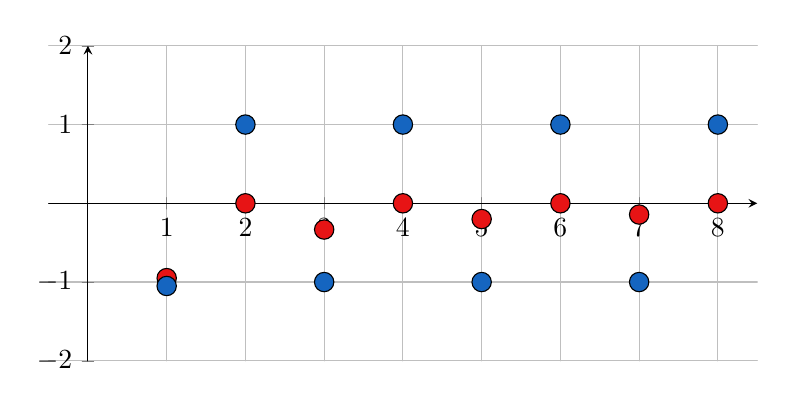
\begin{tikzpicture}[line cap=round,line join=round,>=triangle 45,x=1cm,y=1cm]
        \begin{axis}[
        x=1cm,y=1cm,axis lines=middle,
        ymajorgrids=true,xmajorgrids=true,
        xmin=-0.5,xmax=8.5,ymin=-2,ymax=2,
        xtick={-6,-5,...,12},ytick={-8,-7,...,6},]
        \clip(-6.257075632047947,-8.323024128584796) rectangle (12.3817309640345,6.5690503527635205);
        \begin{scriptsize}
        \draw [fill=rvwvcq] (2,1) circle (3.5pt);
        \draw [fill=rvwvcq] (3,-1) circle (3.5pt);
        \draw [fill=rvwvcq] (4,1) circle (3.5pt);
        \draw [fill=rvwvcq] (5,-1) circle (3.5pt);
        \draw [fill=rvwvcq] (6,1) circle (3.5pt);
        \draw [fill=rvwvcq] (7,-1) circle (3.5pt);
        \draw [fill=rvwvcq] (8,1) circle (3.5pt);
        \draw [fill=exrurv] (2,0) circle (3.5pt);
        \draw [fill=exrurv] (4,0) circle (3.5pt);
        \draw [fill=exrurv] (6,0) circle (3.5pt);
        \draw [fill=exrurv] (3,-0.3333333333333333) circle (3.5pt);
        \draw [fill=exrurv] (5,-0.2) circle (3.5pt);
        \draw [fill=exrurv] (7,-0.14285714285714285) circle (3.5pt);
        \draw [fill=exrurv] (8,0) circle (3.5pt);
        \draw [fill=exrurv] (1,-0.95) circle (3.5pt);
        \draw [fill=rvwvcq] (1,-1.05) circle (3.5pt);
        \end{scriptsize}
        \end{axis}
        \end{tikzpicture}
    \end{figure}
\end{frame}

\begin{frame}
    \begin{zgled}
        Poiščimo primer omejenega zaporedja, ki ni Ces\`{a}ro konvergentno. 
        \visible<2->{Prvi člen naj bo enak $2$.} 
        \visible<3->{Naslednjih nekaj členov bo enakih $-2$. Takih členov mora biti dovolj, da bo aritmetična sredina padla pod $-1$.} 
        \visible<4->{Nato spet dodajmo dovolj členov enakih $2$, da bo aritmetična sredina narasla nad $1$.} 
    \end{zgled}

    \begin{figure}
        \begin{tikzpicture}[line cap=round,line join=round,>=triangle 45,x=1cm,y=1cm]
        \begin{axis}[
        x=0.7cm,y=0.7cm,axis lines=middle,
        ymajorgrids=true,xmajorgrids=true,
        xmin=-0.5,xmax=12.5,ymin=-2.5,ymax=2.5,
        xtick={-2,-1,...,19},
        ytick={-5,-4,...,6},]
        \clip(-2.098760183145331,-5.918856829532279) rectangle (19.334790664437605,6.407246048049231);
        \begin{scriptsize}
        \only<2->{
            \draw [fill=exrurv] (1,1.95) circle (3.5pt);
            \draw [fill=rvwvcq] (1,2.05) circle (3.5pt);
        }
        \only<3->{
            \draw [fill=exrurv] (2,0) circle (3.5pt);
            \draw [fill=rvwvcq] (2,-2) circle (3.5pt);
            \draw [fill=exrurv] (3,-0.6666666666666666) circle (3.5pt);
            \draw [fill=rvwvcq] (3,-2) circle (3.5pt);
            \draw [fill=exrurv] (4,-1) circle (3.5pt);
            \draw [fill=rvwvcq] (4,-2) circle (3.5pt);
        }
        \only<4->{
            \draw [fill=exrurv] (5,-0.4) circle (3.5pt);
            \draw [fill=rvwvcq] (5,2) circle (3.5pt);
            \draw [fill=exrurv] (6,0) circle (3.5pt);
            \draw [fill=rvwvcq] (6,2) circle (3.5pt);
            \draw [fill=rvwvcq] (7,2) circle (3.5pt);
            \draw [fill=exrurv] (7,0.2857142857142857) circle (3.5pt);
            \draw [fill=rvwvcq] (8,2) circle (3.5pt);
            \draw [fill=exrurv] (8,0.5) circle (3.5pt);
            \draw [fill=rvwvcq] (9,2) circle (3.5pt);
            \draw [fill=exrurv] (9,0.6666666666666666) circle (3.5pt);
            \draw [fill=rvwvcq] (10,2) circle (3.5pt);
            \draw [fill=exrurv] (10,0.8) circle (3.5pt);
            \draw [fill=rvwvcq] (11,2) circle (3.5pt);
            \draw [fill=exrurv] (11,0.9090909090909091) circle (3.5pt);
            \draw [fill=rvwvcq] (12,2) circle (3.5pt);
            \draw [fill=exrurv] (12,1) circle (3.5pt);
        }
        \end{scriptsize}
        \end{axis}
        \end{tikzpicture}
    \end{figure}

\end{frame}

\begin{frame}
    \begin{zgled}
        Naj bo $m \in \mathbb{N}$ in $a_1, a_2, \ldots, a_m \in \mathbb{R}$. Zanima nas, kdaj zaporedje $a_1, a_2, \ldots, a_m, a_1, a_2, \ldots$ Ces\`{a}ro konvergira proti $0$. Naj bo $A := a_1 + a_2 + \ldots + a_m$. Ker za vse $k \in \mathbb{N}$ velja $\overline{a}_{km} = \frac{A}{m}$, je enakost $A = 0$ potreben pogoj za $a_n \leadsto 0$. Naj bo torej $A = 0$. Zaporedje delnih vsot zaporedja $(a_n)$ je potem periodično, zato je omejeno. Sledi, da zaporedje aritmetičnih sredin konvergira proti $0$. Torej $(a_n)$ Ces\`{a}ro konvergira proti $0$ natanko tedaj, ko velja $A = 0$.
    \end{zgled}
    %\vspace{100pt}
    \begin{figure}
        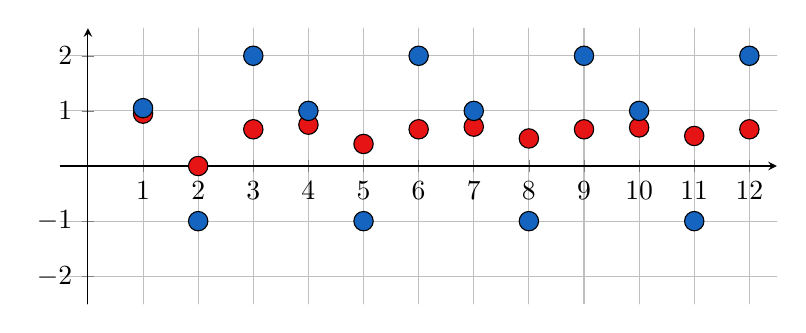
\begin{tikzpicture}[line cap=round,line join=round,>=triangle 45,x=1cm,y=1cm]
        \begin{axis}[
        x=0.7cm,y=0.7cm,axis lines=middle,
        ymajorgrids=true,xmajorgrids=true,
        xmin=-0.5,xmax=12.5,ymin=-2.5,ymax=2.5,
        xtick={-2,-1,...,19},
        ytick={-5,-4,...,6},]
        \clip(-2.098760183145331,-5.918856829532279) rectangle (19.334790664437605,6.407246048049231);
        \begin{scriptsize}
            \draw [fill=exrurv] (1,0.95) circle (3.5pt);
            \draw [fill=rvwvcq] (1,1.05) circle (3.5pt);
            \draw [fill=exrurv] (2,0.0) circle (3.5pt);
            \draw [fill=rvwvcq] (2,-1) circle (3.5pt);
            \draw [fill=exrurv] (3,0.6666666666666666) circle (3.5pt);
            \draw [fill=rvwvcq] (3,2) circle (3.5pt);
            \draw [fill=exrurv] (4,0.75) circle (3.5pt);
            \draw [fill=rvwvcq] (4,1) circle (3.5pt);
            \draw [fill=exrurv] (5,0.4) circle (3.5pt);
            \draw [fill=rvwvcq] (5,-1) circle (3.5pt);
            \draw [fill=exrurv] (6,0.6666666666666666) circle (3.5pt);
            \draw [fill=rvwvcq] (6,2) circle (3.5pt);
            \draw [fill=exrurv] (7,0.7142857142857143) circle (3.5pt);
            \draw [fill=rvwvcq] (7,1) circle (3.5pt);
            \draw [fill=exrurv] (8,0.5) circle (3.5pt);
            \draw [fill=rvwvcq] (8,-1) circle (3.5pt);
            \draw [fill=exrurv] (9,0.6666666666666666) circle (3.5pt);
            \draw [fill=rvwvcq] (9,2) circle (3.5pt);
            \draw [fill=exrurv] (10,0.7) circle (3.5pt);
            \draw [fill=rvwvcq] (10,1) circle (3.5pt);
            \draw [fill=exrurv] (11,0.5454545454545454) circle (3.5pt);
            \draw [fill=rvwvcq] (11,-1) circle (3.5pt);
            \draw [fill=exrurv] (12,0.6666666666666666) circle (3.5pt);
            \draw [fill=rvwvcq] (12,2) circle (3.5pt);
        \end{scriptsize}
        \end{axis}
        \end{tikzpicture}
    \end{figure}
\end{frame}



\section{Ces\`{a}ro zveznost}

\begin{frame}
    \begin{definicija}
        Funkcija $f: \mathbb{R} \rightarrow \mathbb{R}$ je Ces\`{a}ro zvezna v točki $a \in \mathbb{R}$, če za vsako zaporedje $(a_n)$, ki Ces\`{a}ro konvergira proti $a$, zaporedje $(f(a_n))$ Ces\`{a}ro konvergira proti $f(a)$. Pravimo, da je $f$ zvezna, če je zvezna v vsaki točki $a \in \mathbb{R}$.
    \end{definicija}
\end{frame}

\begin{frame}
    \begin{zgled}
        Pokazati želimo, da je vsaka funkcija oblike $f(x) = Ax + B$, kjer sta $A, B \in \mathbb{R}$, Ces\`{a}ro zvezna. 
        \pause

        Naj bo $(a_n)$ poljubno Ces\`{a}ro konvergentno zaporedje in $a$ njegova Ces\`{a}ro limita. Zaporedje $(A a_n + B)$ Ces\`{a}ro konvergira k $A a + B = f(a)$, torej je funkcija $f$ res Ces\`{a}ro zvezna.
    \end{zgled}
    \pause
    \begin{zgled}
        Oglejmo si še primer funkcije, ki ni Ces\`{a}ro zvezna. 
        \pause

        Naj bo $f(x) = x^2$ funkcija. Zaporedje $((-1)^n)$ Ces\`{a}ro konvergira k $0$, zaporedje $(f((-1)^n))$ pa je konstantno enako $1$, zato Ces\`{a}ro konvergira k $1$ in ne k $f(0) = 0$. Torej $f$ ni Ces\`{a}ro zvezna v točki $0$.
    \end{zgled}
\end{frame}

\begin{frame}
    \begin{izrek}
        \label{klaszvez}
        Naj bo $f: \mathbb{R} \rightarrow \mathbb{R}$ funkcija. Naslednje trditve so ekvivalentne.
        \begin{enumerate}
            \item Funkcija $f$ je Ces\`{a}ro zvezna v točki $0$.
            \item Funkcija $f$ je Ces\`{a}ro zvezna.
            \item Funkcija $f$ je oblike $f(x) = Ax + B$ za neki realni števili $A, B \in \mathbb{R}$.
        \end{enumerate}
    \end{izrek}
\end{frame}

\begin{frame}
    \begin{block}{}
        Če je funkcija $f$ Ces\`{a}ro zvezna v točki $0$, je oblike $f(x) = Ax + B$ za neki realni števili $A, B \in \mathbb{R}$.
    \end{block}
    \begin{dokaz}\renewcommand{\qedsymbol}{}
        $(1) \Rightarrow (3): $ Naj bo funkcija $g: \mathbb{R} \rightarrow \mathbb{R}$ definirana s predpisom $g(x) = f(x) - f(0)$. Potem je $g$ Ces\`{a}ro zvezna v točki $0$ in velja $g(0) = 0$. Pokazali bomo, da je $g$ aditivna.
        \pause
        Naj bo $a \in \mathbb{R}$ poljubno realno število. Ker velja $$a, -a, a, -a, a, \ldots \leadsto 0$$ in je $g$ Cesaro zvezna v $0$ velja $$g(a), g(-a), g(a), g(-a), \ldots \leadsto g(0) = 0.$$ 
        \pause 
        Potem mora veljati $g(-a) = -g(a)$. 
    \end{dokaz}
\end{frame}

\begin{frame}
    \begin{block}{}
        Če je funkcija $f$ Ces\`{a}ro zvezna v točki $0$, je oblike $f(x) = Ax + B$ za neki realni števili $A, B \in \mathbb{R}$.
    \end{block}
    \begin{dokaz}\renewcommand{\qedsymbol}{}
        Naj bosta zdaj $b, c \in \mathbb{R}$ poljubni realni števili. Spet vidimo, da velja 
        $$b, c, -(b+c), b, c, -(b+c), \ldots \leadsto 0,$$ zato tudi zaporedje $$g(b), g(c), g(-(b+c)), g(b), \ldots \leadsto 0.$$
        \pause
        Sledi $g(b) + g(c) + g(-(b+c)) = 0$ oziroma $-(g(b) + g(c)) = g(-(b+c))$. 
        \pause 
        Upoštevamo še, da je velja $g(-a) = -g(a)$ za vsak $a \in \mathbb{R}$ in dobimo $g(b) + g(c) = g(b+c)$. Torej je $g$ aditivna.
    \end{dokaz}
\end{frame}

\begin{frame}
    \begin{block}{}
        Če je funkcija $f$ Ces\`{a}ro zvezna v točki $0$, je oblike $f(x) = Ax + B$ za neki realni števili $A, B \in \mathbb{R}$.
    \end{block}
    \begin{dokaz}\renewcommand{\qedsymbol}{}
        Naslednji cilj je pokazati, da velja $g(\lambda x) = \lambda g(x)$ za vse $\lambda \in \mathbb{Q}$ in $x \in \mathbb{R}$. Za primer, ko je $\lambda \in \mathbb{N}$, to sledi neposredno iz aditivnosti. Ker velja tudi $g(0) = 0$ in $g(-a) = -g(a)$, to velja celo za vse $\lambda \in \mathbb{Z}$. 
        \pause

        Naj bo zdaj $\frac{m}{n} \in \mathbb{Q}$ poljubno racionalno število. Velja 
        $$mg(x) = g(mx) = g(n\frac{m}{n}x) = ng(\frac{m}{n}x)$$ 
        oziroma 
        $$\frac{m}{n}g(x) = g(\frac{m}{n}x),$$ 
        kar smo želeli dokazati.
    \end{dokaz}
\end{frame}

\begin{frame}
    \begin{block}{}
        Če je funkcija $f$ Ces\`{a}ro zvezna v točki $0$, je oblike $f(x) = Ax + B$ za neki realni števili $A, B \in \mathbb{R}$.
    \end{block}
    \begin{dokaz}\renewcommand{\qedsymbol}{}
        Pokažimo zdaj, da je $g$ zvezna. Naj bo $(x_n)$ poljubno zaporedje, da je $x_n \rightarrow 0$. Poiščimo zaporedje $(y_n)$, katerega zaporedje aritmetičnih sredin je enako $(x_n)$. 
        \pause
        Očitno mora biti $y_1 = x_1$. Denimo, da smo že definirali $y_1, \ldots, y_n$ in da velja $x_k = \overline{y}_k$ za vse $k \leq n$. Da bo veljalo tudi $x_{n+1} = \overline{y}_{n+1}$ oziroma 
        $$x_{n+1} = \frac{y_1 + \ldots + y_{n+1}}{n+1},$$ 
        moramo vzeti $y_{n+1} = (n+1)x_{n+1} - (y_1 + \ldots + y_n)$. 
        \pause
        
        Tako definirano zaporedje $(y_n)$ res zadošča $x_n = \overline{y}_n$ za vse $n \in \mathbb{N}$.
    \end{dokaz}
\end{frame}

\begin{frame}
    \begin{block}{}
        Če je funkcija $f$ Ces\`{a}ro zvezna v točki $0$, je oblike $f(x) = Ax + B$ za neki realni števili $A, B \in \mathbb{R}$.
    \end{block}
    \begin{dokaz}\renewcommand{\qedsymbol}{}
        Tako definirano zaporedje $(y_n)$ res zadošča $x_n = \overline{y}_n$ za vse $n \in \mathbb{N}$. Ker je $x_n \rightarrow 0$, je $y_n \leadsto 0$ po definiciji, zato iz Ces\`{a}ro zveznosti funkcije $g$ v $0$ sledi $g(y_n) \leadsto g(0) = 0$. Iz tega, kar smo pokazali v prejšnjih odstavkih, potem sledi 
        $$g(x_n) = g(\overline{y}_n) = g(\frac{y_1 + \ldots + y_n}{n}) = \frac{g(y_1) + \ldots + g(y_n)}{n} \rightarrow 0.$$
        Torej je $g$ zvezna v $0$. Ker je $g(x_0 + x) = g(x_0) + g(x)$, je zvezna tudi v vsaki drugi točki $x_0 \in \mathbb{R}$.
    \end{dokaz}
\end{frame}

\begin{frame}
    \begin{block}{}
        Če je funkcija $f$ Ces\`{a}ro zvezna v točki $0$, je oblike $f(x) = Ax + B$ za neki realni števili $A, B \in \mathbb{R}$.
    \end{block}
    \begin{dokaz}
        Naj bo $A = g(1)$. Zvezni funkciji $g$ in $x \mapsto Ax$ se ujemata na $\mathbb{Q}$, ki je gosta podmnožica v $\mathbb{R}$, torej sta enaki. Če vzamemo $B = f(0)$, velja $f(x) = Ax + B$ za vse $x \in \mathbb{R}$. S tem je implikacija dokazana.
        \pause

        \medskip
        $(3) \Rightarrow (2): $ To smo pokazali v zgornjem zgledu.
        \pause

        \medskip
        $(2) \Rightarrow (1): $ Če je $f$ Ces\`{a}ro zvezna, je po definiciji Ces\`{a}ro zvezna tudi v točki $0$.
    \end{dokaz}
\end{frame}


\section{Ces\`{a}ro odvedljivost}

\begin{frame}
    \begin{definicija}
        Funkcija $f: \mathbb{R} \rightarrow \mathbb{R}$ je Ces\`{a}ro odvedljiva v točki $a \in \mathbb{R}$, če obstaja število $f'(a) \in \mathbb{R}$, da za vsako zaporedje $(a_n)$ s členi različnimi od $a$, ki Ces\`{a}ro konvergira proti $a$, zaporedje diferenčnih kvocientov 
        $$(\frac{f(a_n)-f(a)}{a_n-a})$$ 
        Ces\`{a}ro konvergira proti $f'(a)$. 
        \pause

        \medskip
        Številu $f'(a)$ v takem primeru rečemo Ces\`{a}ro odvod funkcije $f$ v točki $a$. 
        \pause

        \medskip
        Pravimo, da je $f$ odvedljiva, če je odvedljiva v vsaki točki $a \in \mathbb{R}$.
    \end{definicija}
\end{frame}

\begin{frame}
    \begin{zgled}
        \label{vseodv}
        Naj bo $f: \mathbb{R} \rightarrow \mathbb{R}$ funkcija oblike $f(x) = Ax^2 + Bx + C$ za neke $A, B, C \in \mathbb{R}$. Naj bo $(a_n)$ poljubno Ces\`{a}ro konvergentno zaporedje s Ces\`{a}ro limito $a$, ki ima vse člene različne od $a$. Velja 
        \begin{align*}
            \frac{f(a_n)-f(a)}{a_n-a} &= \frac{(Aa_n^2 + Ba_n + C)-(Aa^2 + Ba + C)}{a_n-a}\\
            &= \frac{A(a_n-a)(a_n+a) + B(a_n-a)}{a_n-a}\\
            &= A(a_n+a) + B \leadsto 2Aa + B,
        \end{align*}
        torej je $f$ Ces\`{a}ro odvedljiva in je $2Ax + B$ njen Ces\`{a}ro odvod.
    \end{zgled}
\end{frame}

\begin{frame}
    \begin{zgled}
        Naj bo zdaj $f: \mathbb{R} \rightarrow \mathbb{R}$ funkcija s predpisom $f(x) = x^3$. Velja 
        $$(-1)^n \leadsto 0,$$ 
        ampak 
        $$\frac{(-1)^3-0^3}{(-1)-0} = 1 \leadsto 1 \neq 0 = f(0).$$ 
        Torej $f$ ni Ces\`{a}ro odvedljiva v točki 0.
    \end{zgled}
\end{frame}

\begin{frame}
    \begin{lema}
        \label{lema}
        Naj bo $f: \mathbb{R} \rightarrow \mathbb{R}$ funkcija. Naj za vsako zaporedje $(a_n)$ s členi različnimi od $0$, ki Ces\`{a}ro konvergira proti $0$, velja $f(a_n) \leadsto f(0)$. Potem je $f$ Ces\`{a}ro zvezna v točki $0$.
    \end{lema}
\end{frame}

\begin{frame}
    \begin{izrek}
        \label{klasodv}
        Naj bo $f: \mathbb{R} \rightarrow \mathbb{R}$ funkcija. Naslednje trditve so ekvivalentne.
        \begin{enumerate}
            \item Funkcija $f$ je Ces\`{a}ro odvedljiva v točki $0$.
            \item Funkcija $f$ je Ces\`{a}ro odvedljiva.
            \item Funkcija $f$ je oblike $f(x) = Ax^2 + Bx + C$ za neka realna števila $A, B, C \in \mathbb{R}$.
        \end{enumerate}
    \end{izrek}
\end{frame}

\begin{frame}
    \begin{dokaz}\renewcommand{\qedsymbol}{}
        $(1) \Rightarrow (3): $ Definiramo funkcijo $f: \mathbb{R} \rightarrow \mathbb{R}$ s predpisom 
        $$
        g(x) = \begin{cases}
            \frac{f(x)-f(0)}{x}; & x \neq 0\\
            f'(0); & x = 0.
        \end{cases}
        $$
        \pause

        Naj bo $(a_n)$ zaporedje s členi različnimi od $0$, da velja $a_n \leadsto 0$. Potem velja 
        $$g(a_n) = \frac{f(a_n)-f(0)}{a_n-0} \leadsto f'(0) = g(0),$$
        po definiciji Ces\`{a}ro odvoda $f$ v točki $0$. 
        \pause
        
        Po lemi je $g$ Ces\`{a}ro zvezna v točki $0$, zato je po izreku oblike $g(x) = Ax + B$ za neka $A, B \in \mathbb{R}$. Potem pa je 
        $f(x) = xg(x) + f(0) = Ax^2 + Bx + C$ za $C = f(0)$.
    \end{dokaz}
\end{frame}

\begin{frame}
    \begin{dokaz}
        $(3) \Rightarrow (2): $ To smo pokazali v zgornjem zgledu.
        \pause

        \medskip
        $(2) \Rightarrow (1): $ Če je $f$ Ces\`{a}ro odvedljiva, je po definiciji Ces\`{a}ro odvedljiva tudi v točki $0$.
    \end{dokaz}
\end{frame}

\begin{frame}{Literatura}
    \begin{thebibliography}{1}
        \bibitem{1}
        J.~A.~Hocutt in P.~L.~Robinson, \emph{Everywhere Differentiable, Nowhere Continuous Functions}, Amer.~Math.~Monthly \textbf{125} (2018) 923--928.
        \bibitem{2}
        P.~R.~Halmos, \emph{Problems for Mathematicians, Young and Old}, Dolciani Mathematical Expositions \textbf{12}, Mathematical Association of America, Washington, 1991.
    \end{thebibliography}
\end{frame}

\end{document}